\begin{frame}{Эволюция информации Фишера}
\begin{columns}
    \column{0.45\textwidth}
     $$
    \rho(0) = \rho_\mathrm{eq} = \dfrac{ e^{\beta I_z} }{Tr \left\{ e^{\beta I_z} \right\} },
    \quad
    \beta = \dfrac{\hbar \omega_0}{k_{B} T}
    $$
    \vspace{5mm}
    $$ F^{k} \leq \left[ \frac N k \right] k^2 + \left(N - k \left[ \frac N k \right]\right)^2 $$
    \column{0.55\textwidth}
    \begin{figure}
      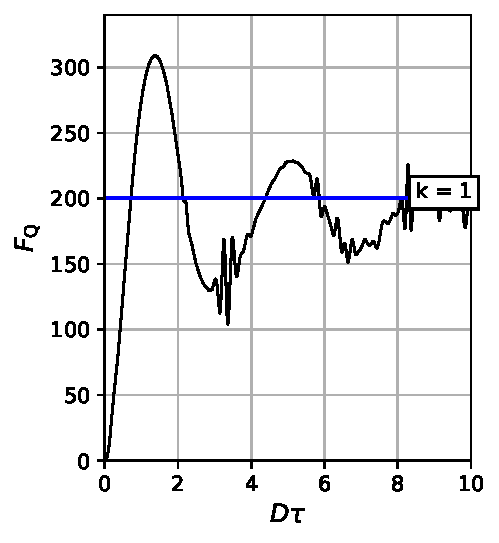
\includegraphics[width=0.65\textwidth]{result-nanopore-eq-m2-by-time-beta0.1.pdf}
      \vspace{-3mm}
      \caption{Зависимость нижней границы информации Фишера от времени. $N = 200$, $\beta = 0.1$.}
    \end{figure}
\end{columns}
\end{frame}
\note{
  Запутанность разрушается при высоких температурах, 
  поэтому в отличие от традиционного подхода, 
  не используется высокотемпературное приближение, 
  и рассмотривается равновесная матрица плотности.

  Для такого начального состояния удалось теретически расчитать спектры МК когерентностей, 
  и вычислить нижнюю границу инфомрацию Фишера. 

  Выше синей линии неравенство для верхней границы информации Фишера нарушается при $k=1$.
  Таким образом в рамках МК спектроскопии ЯМР удается зарегистрировать двух частичную запутанность. 
}

\begin{frame}{Эволюция информации Фишера}
  % \vspace{-5mm}
  % $$
  %   \rho(0) = \rho_\mathrm{eq} = \dfrac{ e^{\beta I_z} }{Tr \left\{ e^{\beta I_z} \right\} },
  %   \quad
  %   \beta = \dfrac{\hbar \omega_0}{k_{B} T}
  % $$
  
  \begin{figure}
    \begin{subfigure}[t]{0.3\textwidth}
      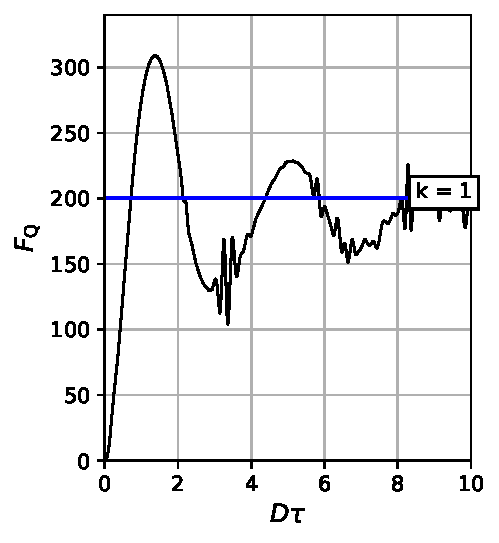
\includegraphics[width=\textwidth]{result-nanopore-eq-m2-by-time-beta0.1.pdf}
      \caption{$\beta = 0.1$}
    \end{subfigure}
    \begin{subfigure}[t]{0.3\textwidth}
      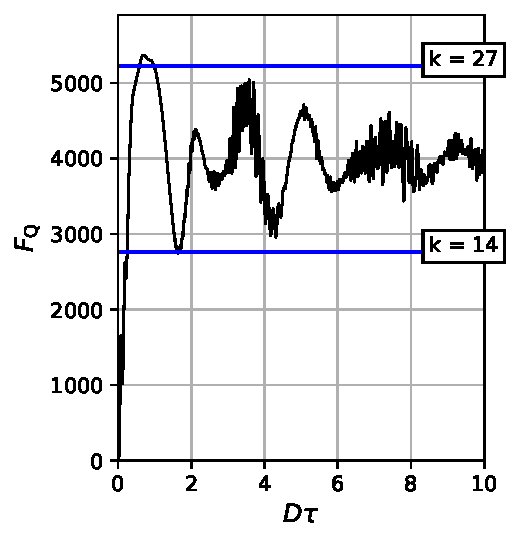
\includegraphics[width=\textwidth]{result-nanopore-eq-m2-by-time-beta0.5.pdf}
      \caption{$\beta = 0.5$}
    \end{subfigure}
    \begin{subfigure}[t]{0.3\textwidth}
      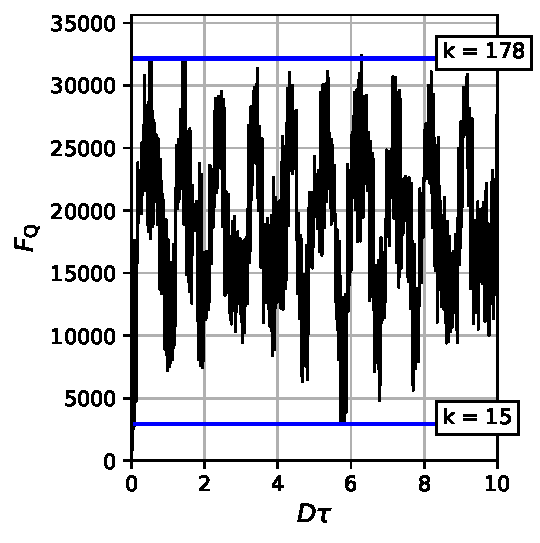
\includegraphics[width=\textwidth]{result-nanopore-eq-m2-by-time-beta3.5.pdf}
      \caption{$\beta = 3.5$}
    \end{subfigure}
    \vspace{-3mm}
    \caption{Зависимость нижней границы информации Фишера от времени. $N = 200$}
  \end{figure}
\end{frame}
\note{
  На сладе представлена зависимость нижней границы информации Фишера от времени при разных температурах. 
  При температуре такой-то регистрируется запутанность такая-то...
}


\begin{frame}{Температурная зависимость многочастичной запутанности}
\begin{columns}
    \column{0.5\textwidth}
    \begin{figure}
    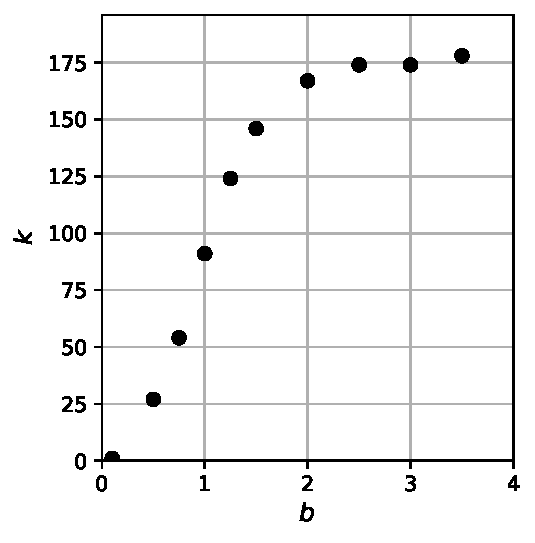
\includegraphics[width=0.65\textwidth]{result-nanopore-eq-nent-by-beta.pdf}
    \caption{Зависимость числа запутанных частиц от обратной температуры. $N = 200$}
    \end{figure}


    \column{0.5\textwidth}
    В начальный момент времени система находится в термодинамическом равновесии:
    $$
    \rho(0) = \rho_\mathrm{eq} = \dfrac{ e^{\beta I_z} }{Tr \left\{ e^{\beta I_z} \right\} },
    \quad
    \beta = \dfrac{\hbar \omega_0}{k_{B} T}
    $$
\end{columns}
\end{frame}
\note{
  Объединяя графики для различных температур удалось получить зависимость количества запутанных спинов от температуры начального состояния. 
  
  При понижении температуры количество запутанных частиц стремительно растет.

  При достаточно низкой температуре почти все спины запутаны друг с другом,
  даже когда начальное состояние не было запутанно. 
}


\begin{frame}{Дипольное упорядочение}
   %  (JETP-20)\footnote{I.D. Lazarev and E.B. Fel'dman , \textit{JETP} \textbf{131}, 5, (2020)}
  \alert{При дипольно упорядоченном начальном состоянии когерентности возникают быстрее:}
  $$
  \rho_i = \frac{1}{Z_i} e^\frac{\hslash\beta_\mathrm{d} \hdz}{k}
  \approx \frac{1}{Z_i}(1 + \frac{\hslash\beta_\mathrm{d}}{k} H_\mathrm{dz}),
  $$
  то есть зеемановская температура низкая, а дипольная --- высокая.
  \begin{block}{Методы создания дипольно упорядоченного состояния}
    \begin{itemize}
      \item  Адиабатическое размагничивание\footnote[frame]{C. P. Slichter and W. C. Holton, Phys. Rev. 122, 1701 (1961)} от большого значения приложенного поля до нуля во вращающейся системе координат.

      \item Двухимпульсный эксперимент Броекаерта-Джинира\footnote[frame]{J. Jeener and P. Broekaert, Phys. Rev. 157, 232 (1967).}.
  \end{itemize}
  \end{block}
\end{frame}
\note{
  Также отдельно был рассмотрено дипольное упорядоченное состояние. 
  Удобным способом создания такого состояния является двух импульсный эксперимент Броекаерта-Джинира.
  В оригинале он не был приспособлен к низким зеемановским температурам,
  но в диссертации доказано, что это возможно и в случай низких зеемановских и высоких дипольных температурах. 

% Был рассмотрен случай низкой зеемановской и высокой дипольной температурами, когда начальное состояние является

%Поэтому представляется целесообразным попытаться непосредственно охладить ядерную спиновую систему, используя то обстоятельство, что она относительно изолировапа от решетки из-за слабости механизмов спин-решеточной релаксации.

%Наиболее прямой метод охлаждения ядерных моментов заключается в их адиабатическом размагничивании от большого значепия приложенного поля до пуля. При обычных условиях охлаждение, получаемое этим способом, оказывается недостаточным.

%Например, адиабатическое размагничивание ядерной спиновой системы, выполняемое, скажем, при температуре решетки $Т_0 = 1$К, начиная с поля $H0 = 25 кЭ$, приводит к конечной температуре $T_f ~ T_0 H_L / H_0$, где величина локального поля $H_L$ состав­ляет несколько эрстед. В этом случае конечная темпера­тура будет порядка $10^{-4}$ К, что по крайней мере на два порядка превосходит требуемое зпачение.

% Эксперимент Броекаерта-Джинира удобнее так как это естественные

% Однако подходы, разработанные для этих исследований, ограничены случаем высоких температур и не могут применяться для изучения многоспиновой запутанности.

% Но нам удалось теоретически доказать что двухимпульсная последовательность Брокаерта – Джинера [17, 19] позволяет получить дипольное упорядоченное состояние даже при низкой зеемановской температуре.

   Также важно отметить, что гамильтониан Hdz частично усредняется быстрой молекулярной диффузией в нанопоре, а усредненный гамильтониан можно записать как
}

% \begin{frame}{Получение дипольно упорядоченого состояния}
% В начальный момент времени система находится в термодинамическом равновесии
% %
% $$
%     \rho(0) = \rho_\mathrm{eq} = \frac{1}{Z}
%     e^{
%       \frac{\hslash \omega_{0}}{k} \alpha_\mathrm{z} I_\mathrm{z}
%       + \frac{\hslash }{k} \beta_\mathrm{d} H_\mathrm{dz}
%     }
% $$
% %
% где $Z$ --- статистическая сумма; \\
% $\alpha_\mathrm{z}$, $\beta_\mathrm{d}$ --- обратные зеемановская и дипольная температуры; \\
% $H_\mathrm{dz}$ --- секулярная часть гамильтониана ДДВ в сильном внешнем магнитном поле;
% $$
%     H_\mathrm{dz} = \frac{D}{2} (3 I^{2}_{z} - I^{2})
% $$
% Нас интересует случай,
% когда зеемановская температура низкая, а дипольная --- высокая
% $$
%     \frac{\hslash \omega_{0}}{k} \alpha_\mathrm{z}\gg 1,
%     \quad\quad
%     \frac{\hslash D}{k}\beta_\mathrm{d} \ll 1
% $$
% \end{frame}
% \note{
%     В начальный момент времени ...
%     И мы уже рассмотрели этот случай в 19 году.
%     Однако в случае дипольного упорядочения когерентности...
%     А как я говорил, дисперсия распределеяня когерентностей связана с количеством запутанных частиц.
% }


\begin{frame}{Эволюция информации Фишера}
  \begin{figure}
    \begin{subfigure}[t]{0.3\textwidth}
    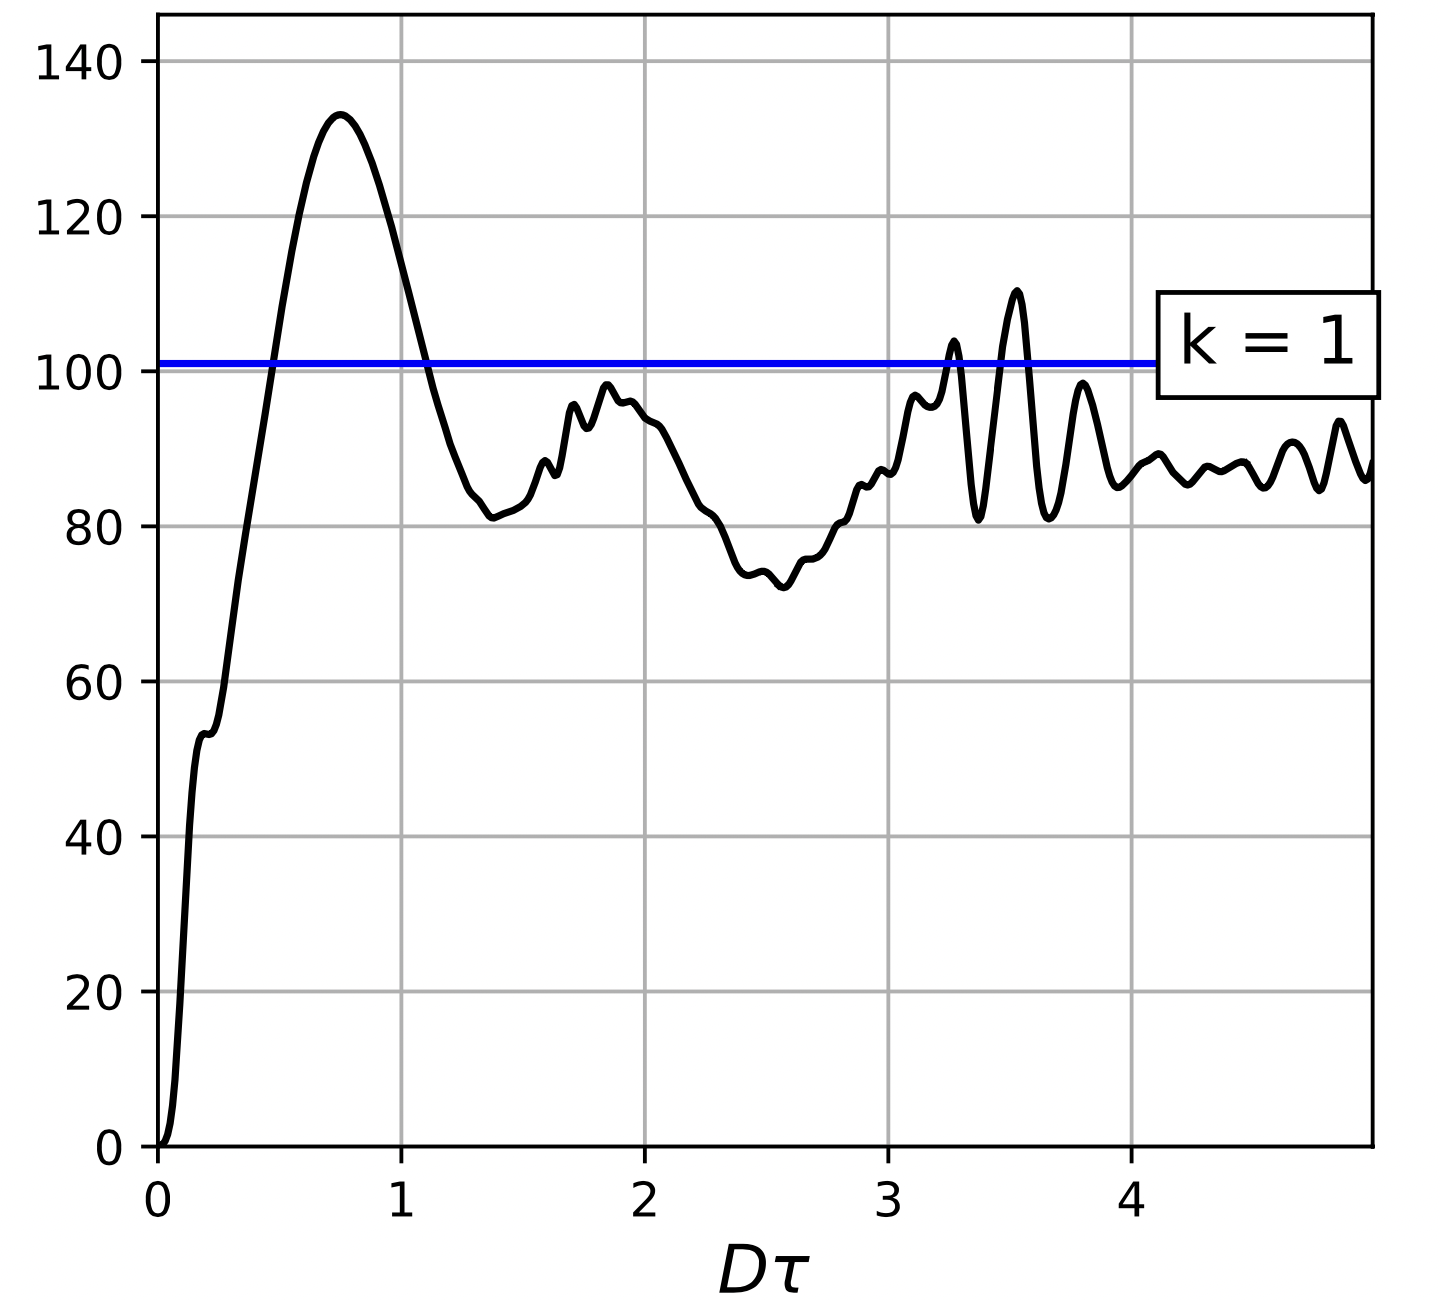
\includegraphics[width=\textwidth]{src/figures/result-nanopore-do-m2-by-time-n101-beta1.png}
    \caption{$T = 6 \times 10^{-4}$ K}
    \end{subfigure}
    \hfill
    \begin{subfigure}[t]{0.3\textwidth}
      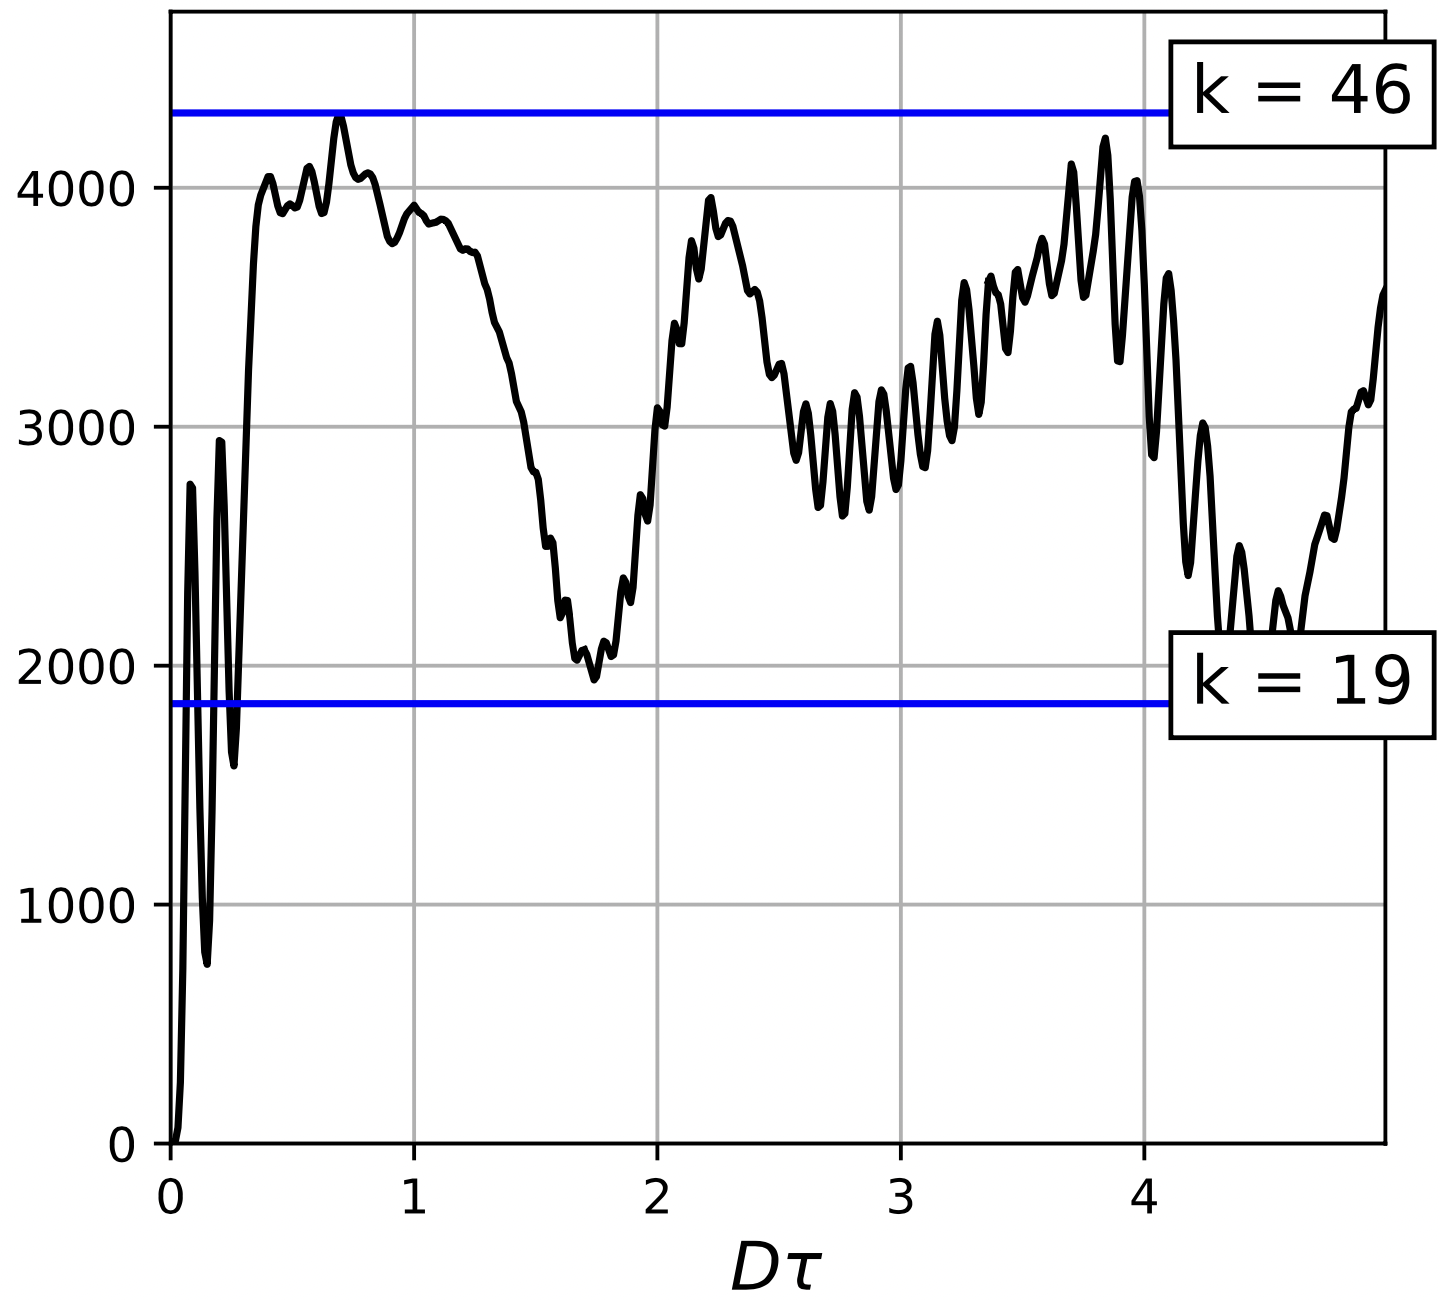
\includegraphics[width=\textwidth]{result-nanopore-do-m2-by-time-n101-beta2.png}
      \caption{$T = 3.2 \times 10^{-4}$ K}
    \end{subfigure}
    \hfill
    \begin{subfigure}[t]{0.3\textwidth}
      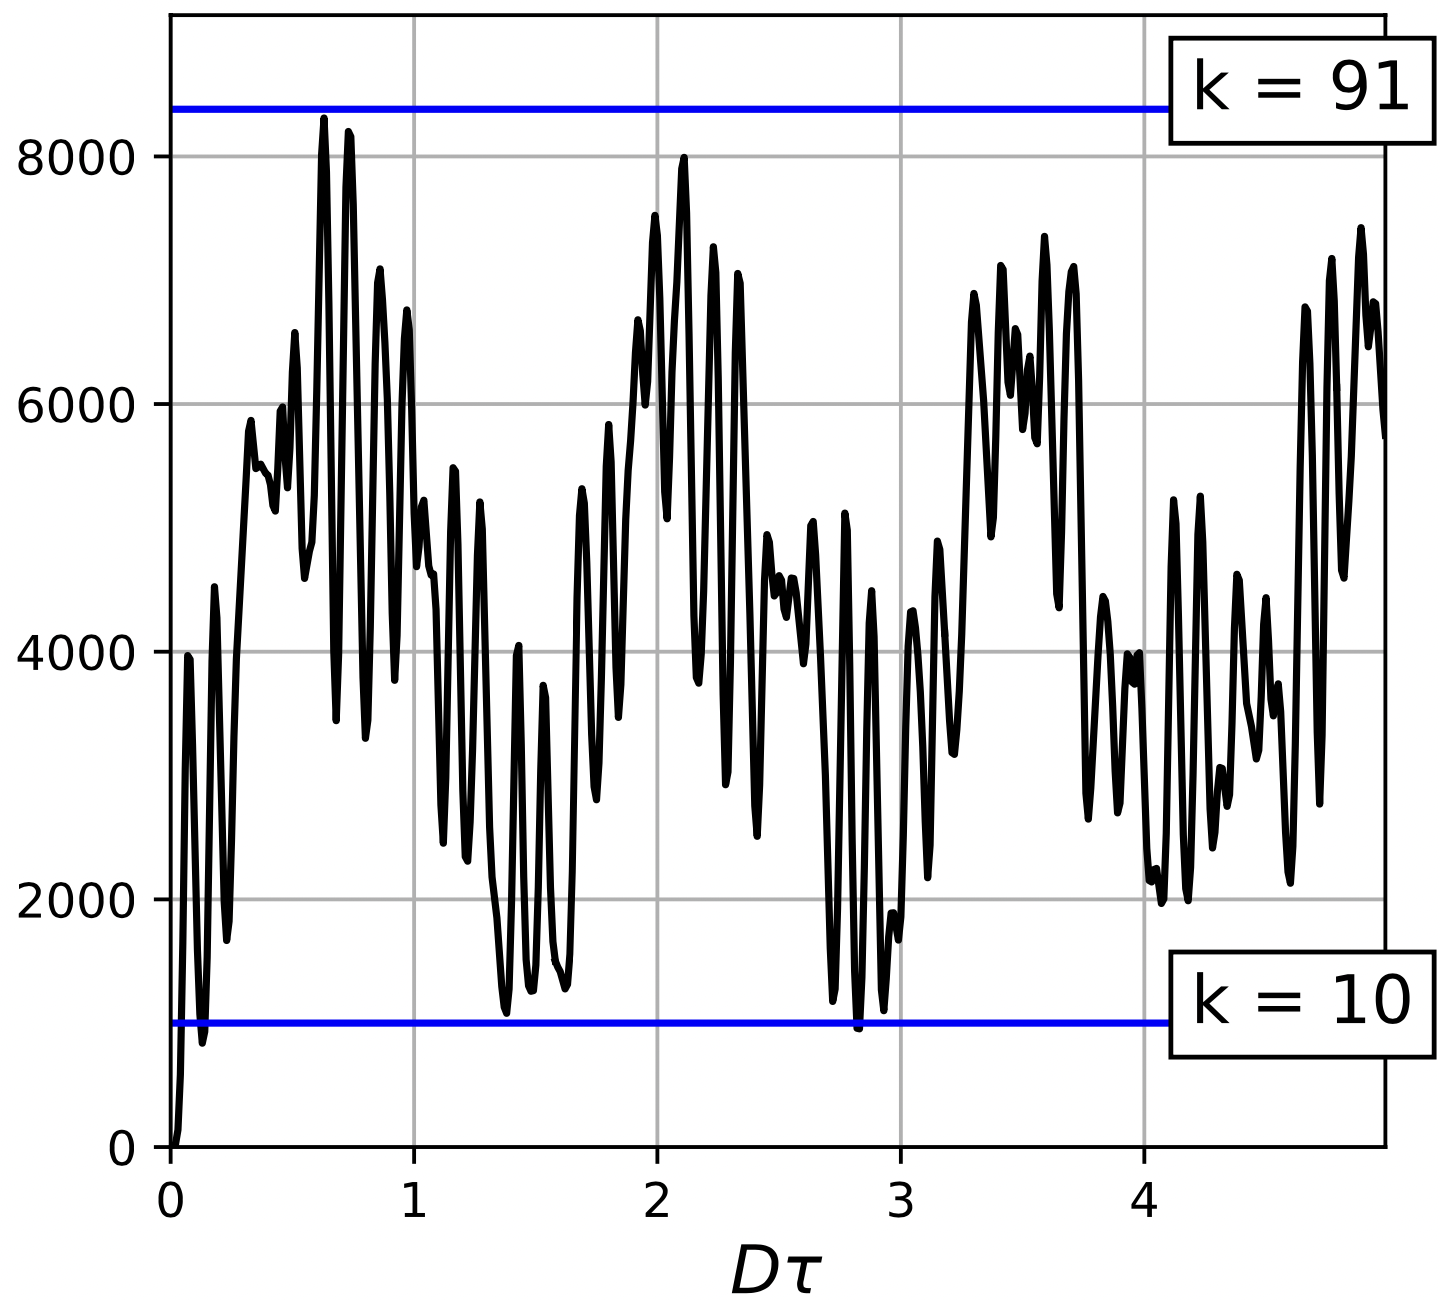
\includegraphics[width=\textwidth]{result-nanopore-do-m2-by-time-n101-beta3.png}
      \caption{$T = 4.8 \times 10^{-5}$ K}
    \end{subfigure}
    \caption{Зависимости нижней границы квантовой информации Фишера $F_Q = 2M_2$ от безразмерного времени $D\tau$ при $N = 101$.}
  \end{figure}
\end{frame}
\note{ 
    Для такого начального состояния удалось тоже расчистать динамику второго момента МК спектра ЯМР. 
    На слайде зависимости ниженй границы информации фишера при различных температурах. 
    % Нам удалось решить динамику для этой системы и изучить систему при разных значения температуры и размера системы.
}

\begin{frame}{Дипольное упорядочение}
    \begin{figure}
    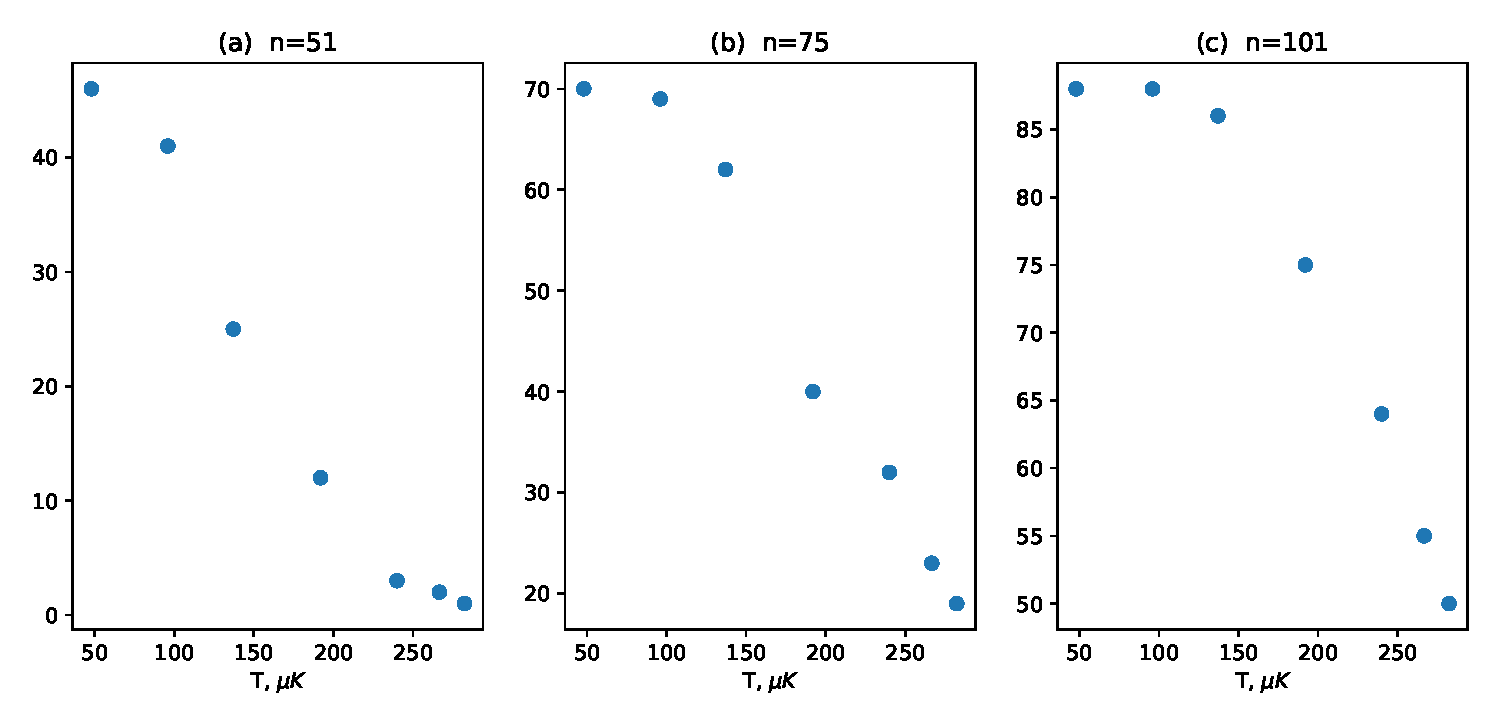
\includegraphics[width=0.85\textwidth]{result-nanopore-do-nent-by-beta-n51-n75-n101.eps}
    \caption{
      Зависимости минимального количества числа запутанных частиц,
      усредненного по времени эволюции, от температуры.
     }
    \end{figure}
\end{frame}
\note{
  По аналогии объединяя графики получены зависимости оценки количества запутанных частиц от температуры для разного количества частиц в системе.  
  % мы хотели поймать скачак количества запутанных состояний, поэтому рассмотрели упорядочение

  % Максимальное количество запутанных спинов при одинаковой температуре увеличивается, когда увеличивается число спинов в нанопоре, потому что система в нанопоре становится плотнее.
}
